%!TEX root = ../thesis.tex

\subsection{提案モデルの識別可能性}

本節では、前節で定義したDAGモデルの識別可能性を証明する
提案モデルは、連続変数と離散変数とが混在することを許容するDAGモデルであるため、
その特殊形として、全てが連続変数であるモデルや全てが離散変数であるモデルを考えることも可能である。
全てが連続変数である場合は、LiNGAM\cite{Shimizu2006-yu}と同様となる。
つまり、全てが連続変数である場合の識別可能性は既に証明されている\cite{Shimizu2006-yu}。
また、全てが離散変数である場合は、QVF-DAGモデル\cite{Park2017-hw}と同様となる。
つまり、全てが離散変数である場合の識別可能性も既に証明されている\cite{Park2017-hw}。
そこで以下では、観測変数集合に連続変数と離散変数の両方が含まれる場合についてのみ述べる。
まず、証明の方針について直感的な理解を得るために、
図\ref{fig:ex_prop_bivariate}のようなDAGモデルを用いて
2変数モデルを用いてその識別可能性を示す。
ここで$X$は連続変数、$Y$は離散変数であるとする。

\begin{itemize}
  \item $G_1 \colon X_1 \sim \mathit{Poisson}(\lambda_1),
         \quad X_2 \sim \mathit{Poisson}(\lambda_2) \quad$ ただし、$X_1$と$X_2$は独立

  \item $G_2 \colon X_1 \sim \mathit{Poisson}(\lambda_1),
         \quad X_2|X_1 \sim \mathit{Poisson}(g_2(X_1))$

  ただし、$g_1$と$g_2$は非退化な任意の関数である。
  $(g_1, g_2 \colon \mathbb{N} \cup \{ 0 \} \rightarrow \mathbb{R}^+)$
\end{itemize}

\begin{figure}[h]
  \centering
  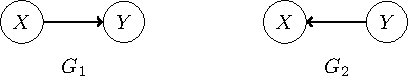
\includegraphics{./picture/prop_bivariate.pdf}
  \caption{2変数のDAGモデル}
  \label{fig:ex_prop_bivariate}
\end{figure}
